% This is a sample document using the University of Minnesota, Morris, Computer Science
% Senior Seminar modification of the ACM sig-alternate style. Much of this content is taken
% directly from the ACM sample document illustrating the use of the sig-alternate class. Certain
% parts that we never use have been removed to simplify the example, and a few additional
% components have been added.

% See https://github.com/UMM-CSci/Senior_seminar_templates for more info and to make
% suggestions and corrections.

\documentclass{sig-alternate}
\usepackage{color}
\usepackage[colorinlistoftodos]{todonotes}
\usepackage{algorithm2e}

%%%%% Uncomment the following line and comment out the previous one
%%%%% to remove all comments
%%%%% NOTE: comments still occupy a line even if invisible;
%%%%% Don't write them as a separate paragraph
%\newcommand{\mycomment}[1]{}

\begin{document}

% --- Author Metadata here ---
%%% REMEMBER TO CHANGE THE SEMESTER AND YEAR AS NEEDED
\conferenceinfo{UMM CSci Senior Seminar Conference, December 2017}{Morris, MN}

\title{Thread Scheduler Efficiency Improvements \\ for Multicore Systems [Draft]}

\numberofauthors{1}

\author{
% The command \alignauthor (no curly braces needed) should
% precede each author name, affiliation/snail-mail address and
% e-mail address. Additionally, tag each line of
% affiliation/address with \affaddr, and tag the
% e-mail address with \email.
\alignauthor
Daniel C. Frazier\\
	\affaddr{Division of Science and Mathematics}\\
	\affaddr{University of Minnesota, Morris}\\
	\affaddr{Morris, Minnesota, USA 56267}\\
	\email{frazi177@morris.umn.edu}
}
\maketitle

\todo[inline]{This is an incomplete Draft.}

\begin{abstract}
[Abstract text]
\end{abstract}

\keywords{Scheduling; thread migration; multicore; multiprocessing; lock contention; last-level cache misses}

\section{Introduction}
\label{sec:intro}

Thread scheduling is a problem that has been around since the 1960s. By the early 2000s, thread scheduling was commonly believed to be solved in the Linux community. However, with the rising popularity of multiprocessor multicore systems and the rapidly developing requirements driven by new hardware, the problem space has become considerably more complex. This paper will describe some newly found issues currently present in the Linux scheduler, their fixes, and two recent developments. All of which substantially improve the efficiency of average programs and improve efficiency for certain programs by up to 138 times.~\cite{Lozi:2016}

\section{Background}
\label{sec:bg}

In this section, we will broadly establish how threading, scheduling, and caching works. We will establish causes of cache misses in the execution of programs using the current Linux thread scheduler. We will establish information necessary to understand the recent developments made to improve thread scheduling for multiprocessor and multicore systems. The first improvement to these performance problems depends on understanding four flaws in the current implementation of the load balancer for the Linux thread scheduler~\cite{Lozi:2016}. The other two improvements involve reducing lock contention between threads by employing new scheduling techniques~\cite{HeeseungEtal:2017,KumarEtal:2014}.

\subsection{Threads and Scheduling}
\label{sec:threads}
Using any modern computers, there is an expectation that the operating system is running at all times (largely in the background) and that multiple user programs and system programs should be able to run concurrently. Modern computer programs also often need to run more than one independent task at one time. This can be accomplished by employing \emph{threads} or  making the program \emph{multithreaded}. Programs that involve long independent computations or programs with a graphical interface often benefit from employing threads.

For example, imagine an image editing program that can apply an expensive filter operation. If the program wasn't multithreaded, the user interface and the filter operation would be executed in the same thread (same \emph{context}). When instructing the program to execute the filter on a large image, the user interface wouldn't be able to respond to any events (like clicking the mouse) until the filter operation was finished. To make the program more responsive, separate the user interface into its own thread and employ more threads when the user initiates an expensive operation.
	
Threads are tied to the \emph{processes} that spawn them. A process always has at least one thread. Processes are typically independant of each other while threads exist within a process. \emph{Context switching} within a CPU is the process of storing and restoring the state of a process or thread so that execution can be paused or resumed. A processes state consists of resources that each of its threads should have access to. These resources are: compiled code and data, sockets, file handles, and logistical information stored in the \emph{process control block} such as processor privileges and what IO devices have been allocated to this process ~\cite{WikiProcessControlBlock,WikiThreads}. A thread's state consists of a stack, a clone of the CPUs registers, and on some systems, extra storage for thread-local global variables~\cite{WikiThreads,WikiThreadLocalStorage}. Context switching is typically fastest between threads within a process because a bulk of the data that is required to be available, the resources, is already available.~\cite{WikiThreads} 

The ~\emph{scheduler} is the part of the operating system that is responsible for managing and distributing the CPU runtime which each of these processes and their respective threads receive. New threads and processes are added to the scheduler when they are made.~\cite{Lozi:2016}

\subsection{Completely Fair Scheduler (CFS)}
\label{sec:cfs}

Scheduler implementations vary per operating system. The scheduler used in Linux is called the Completely Fair Scheduler (CFS). We will discuss the CFS as presented in Lozi, Lepers, Funston, Gaud, Quéma and Fedorova~\cite{Lozi:2016}. The CFS is an implementation of the weighted fair queuing (WFQ) scheduling algorithm. The goal of the WFQ is to divide available CPU cycles among threads, prioritizing more cycles for threads with larger weights.

Threads that are running accumulate \emph{vruntime}, which is the runtime of a thread divided by its weight. Once a thread's vruntime is greater than the amount of runtime that the thread was scheduled for and there is another thread waiting to take this thread's place, the running thread is preempted from the CPU. A thread may also become preempted if another thread with a smaller vruntime awakens. Threads are organized in a priority queue called a \emph{runqueue}. This priority queue implementation uses a self-balancing binary tree called a red-black tree in which the nodes are threads and the leftmost node is always the thread with the smallest vruntime.~\cite{Lozi:2016}

In order for the scheduler to work on multiple cores, each core must have its own runqueue. If all cores shared one runqueue, each core would need to make frequent synchronous requests for process and thread state information from other cores~\cite{Lozi:2016}. For the scheduler to function properly and efficiently, it must keep each of the runqueues balanced. If runqueues are not balanced, then a core is left idle and needs to request work from another core to keep busy. External calls between cores are expensive and should be minimized. Most schedulers, including the CFS, run a load-balancing algorithm that tries its best to keep runqueues balanced. Load-balancing was simple for single-core systems, but with multi-core systems, bugs have found their way into the system and persist even until today

\begin{quote}
Our recent experience with the Linux scheduler revealed that the pressure to work around the challenging properties of modern hardware, such as non-uniform memory access latencies (NUMA), high costs of cache coherency and synchronization, ... resulted in a scheduler with an incredibly complex implementation. As a result, the very basic function of the scheduler, which is to make sure that runnable threads use idle cores, fell through the cracks.~\cite{Lozi:2016}
\end{quote}

Before we can meaningfully discuss these bugs, we must first understand how cache exists on most multicore systems, how cache coherency and synchronous accesses effect performance, and a few other related system performance concepts.

\todo[inline]{Something crucial that I don't yet have an answer for is that reading through Lozi, they never mention what CFS looks like on Multiprocessor machines, only what it looks like on a multicore processor. But then in the description of NUMA nodes there is cache built on each pair of \emph{cores}, not processors. The Systems book seems to imply that cache is commonly integrated per processor but it doesn't specify that it is last-level cache. Is L1 cache primarily found on/between cores or processors? Followup question, is an instance of the CFS ran for each processor? How does the scheduler decide which processor threads are assigned to on Linux systems?}

\todo[inline]{RIGHT Each group of n cores is a scheduling domain, and as such, a processor and groups of processors can be scheduling domains, which the CFS/Load balancer algorithms do support. I'm still not entirely clear on which cache tends to reside, though.
}

\subsection{Cache on NUMA Systems}
\label{sec:cache}

When a program is running, memory is stored in the RAM. The RAM exists far away from the CPU relative to the cache. Imagine a program that sums up an array of one million integers and they all fit into RAM. It would be very slow for the CPU to request from the RAM integers one at a time. Cache allows us to speed up this process by taking a chunk of data that the system predicts will be used frequently, and migrating it from the RAM into cache.

In a \emph{non-uniform memory access (NUMA)} system, there are many levels of cache and they exist in a hierarchy. At the lowest level of the hierarchy is a grouping of some amount of cores that together create a \emph{NUMA node}. The number of levels in a system's hierarchy depend on the hardware. On the machine used in Lozi et al. there were 32 cores, eight cores per NUMA node. See Figure~\ref{fig:NUMA}.~\cite{Lozi:2016} NUMA nodes are the most atomic level of cache present on a modern computing system that employs NUMA. The \emph{last level cache (LLC)} is labeled L1 and larger caches in the hierarchy are L2, L3, etc. NUMA nodes are L1 cache and are last level cache. Last level cache has the fastest data lookup times from a core because it is located nearer to the CPU. If a unit of cache is not found in an L1 cache, it is called an \emph{LLC miss} and the data is searched for in the next level of cache. If the data can not be found in any level of cache, it is just called a \emph{cache miss} and external memory is consulted for the data. Moving data closer to the CPU improves \emph{locality} because it makes the data more ``local'' to where it needs to be. Improving locality improves performance because the system works less hard to load the data it needs.~\cite{WikiCache}

\begin{figure}
\centering
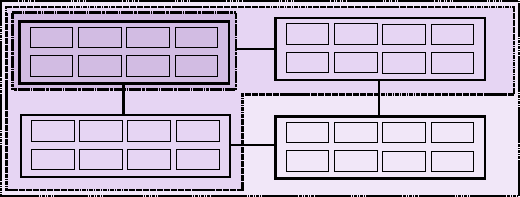
\psfig{file=NUMA.pdf,width =3in}
\caption{32-core machine with four NUMA nodes. It only takes two hops to get from any core to another node. The shades represent scheduling domains relative to the first core.  From Lozi et al.~\cite{Lozi:2016}}
\label{fig:NUMA}
\end{figure}

An important property of a system that employs cache is that it should be \emph{cache coherent}. When data is written into cache, it must propogate to all levels of cache accessible to the processor that issued the write. There are increasing read/write latencies for each level of cache away from a processor. Any changes to a portion of data in an L1 cache must propogate to L2, L3, etc. A system that is cache coherent is a system that satisfies the invariant that any data that is read that pertains to a certain portion of cached data must be consistent with the most recent write to that portion of data. This becomes a difficult problem in the instance that two different cores have both cached the same portion of data and are making concurrent reads and writes to this data. Some processor setups involve sharing cache between processors. Cache sharing is not ideal, though, because a mechanism must be emplaced to arbitrate \emph{synchronous} access to shared data (synchronous access will be defined in the following subsection.) Further, per-proccessor cache can be physically integrated into processors in order to minimize cache access latency where shared cache does not benefit. The most common approach to maintain strict consistency in cache is to somehow \emph{invalidate} cache entries. How cache invalidation works is out of the scope of this paper~\footnote{For the curious, see Section 10.2.4 in Part II of Principles of Computer System Design by Saltzer, Jerome and Kaashoek, M. Frans for more information on methods of cache invalidation.}.~\cite{Systems}

\todo[inline]{Should this transition better, or does the parenthesis in the paragraph above prepare the reader enough to know what to expect in the next section? Also, create or find a Figure describing what a cache hierarchy could look like.}

\subsection{Synchronicity, Locks and Lock Contention}
\label{sec:locks}





\section{Methods}
\label{sec:methods}

So far we have established what threads are, how cache works and where it resides on NUMA systems and how the CFS scheduler works. Now, we will discuss three bugs Lozi et al. found in the CFS load-balancer and their fixes, which substantially improved scheduler efficiency. Later, we will show two more solutions that improve efficiency for certain kinds of programs running on multiprocessor multicore NUMA systems.

\subsection{Load-Balancing the CFS}
\label{sec:loadbalance}

As we mentioned in Section \ref{sec:cfs}, modifications were made to the CFS that introduced bugs that caused processors to remain idle even when there were threads available. Work by Lozi et al. has identified four bugs that were responsible for this behaviour. These bugs have remained hidden because, while they corrode performance, they are not obvious. They do not make programs freeze or crash and their effects only last a few hundred milliseconds at a time, which is too short for common performance tools like \textbf{top} to detect. Lozi et al. designed new tools that observe the Linux scheduler more closely. Using these tools helped these researches locate the problems.~\cite{Lozi:2016}

In order to understand these bug fixes, as described in Lozi et al., we must explain a simplified version of the CFS load balancer.~\cite{Lozi:2016}

\subsubsection{Load Metric}
\label{sec:loadmetric}

The load-balancing algorithm tracks a metric called \emph{load} to best distribute threads to cores. Defining what load should be is tricky. Balancing load such that each core has the same amount of threads is not ideal because threads have priorities, and if all of the high-priority threads happened to be placed on one core while all low-priority threads were placed on another, the low-priority threads would be receiving much more runtime than they should be in relation to the high-priority threads. Balancing load such that each core has roughly the same amount of weight is not ideal either, because, if there was one thread that was nine times more important than nine low-priority threads, that important thread would be left on a core all alone. That seems acceptable, but consider the case that this high-priority thread sleeps a lot. Its core would be left idle for an unnacceptable amount of time. The idle core would need to ask other cores for more work to keep busy in the downtime, which is an expensive operation for both cores involved.~\cite{Lozi:2016}

The current implementation of CFS uses a combination of a thread's weights and average CPU use divided by the amount of all threads in the parent process for the load metric. It divides by the amount of all threads in the parent process in order to remain fairness so that two processes that have different amounts of threads of the same priority still get equal runtime.~\cite{Lozi:2016}

\subsubsection{Load-Balancing Algorithm}
\label{sec:loadbalancealg}

Cores exist in the hierarchy where each level is called a \emph{scheduling domain}. The groups within each level are based on how cores share resources with the machine. The lowest level of scheduling domain is a single core. In the machine described in Section~\ref{sec:cache} there were 32 cores (first level), four NUMA nodes (second level), the third level was formed by groupings of nodes that are within one hop of each other, and the final level is all of the nodes as one unit.
The load-balancing algorithm is run for each scheduling domain starting at the first level's scheduling domain and ending on the final level's scheduling domain. One core per scheduling domain is responsible for performing the load-balancing for that domain.

\todo[inline]{finish}

\subsection{Bugs and Fixes for the CFS}
\label{sec:cfsbugs}

Now that we know how the load balancer functions, we will now dive into the bugs that occur as a result of the complex, strict requirements that have built up over time on the CFS.

\subsubsection{The Group Imbalance bug}
\label{sec:cfsfault_grpimbalance}

This bug was first encountered when the researchers were compiling the Linux kernel with \textbf{make} on 64 cores and also had two R programs running, each of which was launched from different ssh connections on three different ttys. ~\cite{Lozi:2016}

\subsubsection{The Scheduling Group Construction bug}
\label{sec:cfsfault_grpconstruct}



\subsubsection{The Overload-on-Wakeup bug}
\label{sec:cfsfault_overload}

\subsubsection{The Missing Scheduling Domains bug}
\label{sec:cfsfault_missingsched}

This bug is actually something that was already fixed but regressed on Linux kernel version 3.19 (and later) when an important line of code was removed in a refactor that causes the system to misrepresent the amount of scheduling domains that are available for assigning threads to. This ended up causing load-balancing to never happen, meaning processes, subprocesses and their threads to stop looking for other NUMA nodes to assign themselves to. Nodes that do not have any threads will never receive threads and nodes that do have threads will accumulate all of the spawned threads.

This bug required that one of the cores become disabled and re-enabled. So while rare, reintroducing the removed line of code increased efficiency in a certain tested program by a maximum of 138 times.~\cite{Lozi:2016}

\subsection{Shuffler}
\label{sec:shuffler}

The CFS does not differentiate between threads of a single-threaded program versus the threads of a multithreaded program. This prevents the scheduler from using that metadata in its thread distribution mechanism. The following thread scheduler named \emph{Shuffler} by Kumar, Rajiv, Laxmi and Bhuyan takes this into account.~\cite{KumarEtal:2014}

Performance of multithreaded applications on multicore, multiprocessor systems with high lock contention is dependant on the distribution of those threads across processors. The Shuffling approach is for the scheduling algorithm to take into account what threads are contending for locks on what processors and migrate threads to share processors. The Shuffling Framework operates by first finding the expected arrival time of locks on threads. Then it sorts these threads by their expected arrival times and groups them in as many groups as there are processors. It continues by distributing these groups of threads into its own respective processors. The migration of threads between processors is costly, but the threads that are contending for locks during that time are not doing any useful work anyway. In addition, contending threads that are co-located in one processor can share data much faster and avoid LLC misses. For these reasons it is preferable to migrate the whole thread rather than its data and the lock. This will be shown in the performance section.~\cite{KumarEtal:2014}

For the first step of the algorithm, it finds the expected arrival time of threads. The \textit{lock time} of a thread is measured by the percent of time it spends waiting for locks. There exists a daemon thread that contains a data structure which maps threads to their lock times and processor ids. For the monitor, we must choose a rate to sample lock acquiring times at (lock arrival times) and a rate to perform thread migration (shuffling). Kumar et al. used prstat, a utility to report active processor statistics~\cite{prstat}, to monitor lock arrival times. They found that finer sampling rates allow for detailed monitoring but also more overhead. They also found that for sampling rates less than 200 ms, the overhead was significantly higher. For a lock sampling rate of 200 ms the process of sampling took less than 1\% system time. The Shuffling interval was chosen by experimentation. They tested various shuffling intervals on 20 programs and chose 500 ms.

On an iteration of the grouping-forming procedure (every 200 ms), the daemon checks the total amount of time that was spent resolving locks on each thread and if that time exceeds a preset limit, then groups are formed again.

On an iteration of the shuffling procedure (every 500 ms), shuffling checks to make sure that if any threads aren't on processors that they were grouped to, they are migrated. Threads that are already on the processor that they were assigned to do not migrate. If the way that threads interacted with eachother doesn't change, the shuffling step is effectively skipped.~\cite{KumarEtal:2014}

\begin{algorithm}
	\SetKwInOut{Input}{input}\SetKwInOut{Output}{output}
	\Input{N: Number of threads;\\
	C: Number of Processors.}

	\Repeat{application terminates}{
		$\textbf{i. Monitor Threads}$ -- sample lock times of N threads.\\
		\If{lock times exceed threshold}{
			$\textbf{ii. Form Thread Groups}$ -- sort threads according to lock times and divide them into C groups. \\
			$\textbf{iii. Perform Shuffling}$ -- shuffle threads to establish newly computed thread groups.
		}
	}			

	\caption{The Shuffling Framework
	as presented in Kumar et al.~\cite{KumarEtal:2014}}\label{euclid}\label{alg:shuffler}
\end{algorithm}

Now that we know how the Shuffling Framework works, let's review the results that implementing it gives us.

\subsubsection{Shuffler Performance}
\label{sec:shuf_performance}

Kumar et al. defines LLC miss rate as the last level cache misses per thousand instructions (MPKI).~\cite{KumarEtal:2014}.

We studied the lock times of 33 programs on a 64-core, 4-processor machine running Oracle Solaris 11. We identified 20 of those programs that experienced overall high lock times and used those programs to compare shuffling versus the standard scheduler.~\cite{KumarEtal:2014}

\todo[inline]{expand, relay more results! Transition cleanly.}


\subsection{FLSCHED for Xeon Phi Manycore Processor}
\label{sec:flsched}


\todo[inline]{write section..}

[Body text]

\subsubsection{Lockless Thread Scheduler}
\label{sec:flsched_about}

\cite{Lozi:2016, HeeseungEtal:2017}
~\cite{KumarEtal:2014}

\subsubsection{FLSCHED Perfomance}
\label{sec:flsched_performance}

[Body text]

\section{Conclusions}
\label{sec:conclusions}

[Conclusion text]
\todo[inline]{After other sections are done write conclusions and introduction.}

\section*{Acknowledgments}
\label{sec:acknowledgments}


% The following two commands are all you need in the
% initial runs of your .tex file to
% produce the bibliography for the citations in your paper.
\bibliographystyle{abbrv}
\bibliography{scheduling}  
% Remember to run:
% latex bibtex latex latex
% to resolve all references

\end{document}
